% Optimal-transport flow matching (OT-FM, i.e. OT-CFM) for the unpaired PYTHIA ->
% JEWEL jet translation (FLOW_NOTES.md, "PYTHIA -> JEWEL translation pilot").
% Numbers: docs/flow/translation/otfm/*.csv (translation_report.py) via
% tables/otfm_*.tex (translation_tables.py --deck otfm); figures:
% docs/flow/translation/deck_otfm/*.png (translation_deck_figs.py). Build:
%   cd docs/flow/translation/slides && ~/pyext/tectonic_env/bin/tectonic translation_otfm.tex
\documentclass[aspectratio=169,10pt]{beamer}
\usetheme{default}
\setbeamertemplate{navigation symbols}{}

\usepackage{booktabs}
\usepackage{graphicx}
\usepackage{xcolor}
\usepackage{tikz}
\usetikzlibrary{positioning,arrows.meta}
\graphicspath{{../deck_otfm/}}

% ink and series colours of the figures (blue / violet: colour-vision safe)
\definecolor{ink}{HTML}{0B0B0B}
\definecolor{ink2}{HTML}{52514E}
\definecolor{muted}{HTML}{898781}
\definecolor{rule}{HTML}{E1E0D9}
\definecolor{cOT}{HTML}{2A78D6}
\definecolor{cRJ}{HTML}{4A3AA7}
\definecolor{wash}{HTML}{F4F3EF}

\setbeamercolor{normal text}{fg=ink}
\setbeamercolor{frametitle}{fg=ink}
\setbeamercolor{title}{fg=ink}
\setbeamercolor{subtitle}{fg=ink2}
\setbeamercolor{date}{fg=muted}
\setbeamercolor{itemize item}{fg=muted}
\setbeamercolor{itemize subitem}{fg=muted}
\setbeamercolor{enumerate item}{fg=ink2}
\setbeamerfont{frametitle}{size=\Large,series=\bfseries}
\setbeamerfont{title}{size=\LARGE,series=\bfseries}
\setbeamertemplate{itemize items}{\raisebox{0.15em}{\scalebox{0.7}{$\blacksquare$}}}
\setbeamertemplate{itemize subitem}{--}
\setbeamersize{text margin left=1.5em,text margin right=1.5em}
\setbeamertemplate{frametitle}{\vspace{0.6em}\insertframetitle\par\vspace{-0.2em}%
  {\color{rule}\rule{\textwidth}{0.6pt}}}
\setbeamertemplate{footline}{\hfill{\scriptsize\color{muted}%
  \insertframenumber\,/\,\inserttotalframenumber}\hspace{1.5em}\vspace{0.9em}}

% line keys in the series colours, then the name in ink
\newcommand{\keyot}{{\color{cOT}\rule[0.25em]{1.1em}{1.6pt}}\,}
\newcommand{\keyrj}{{\color{cRJ}\rule[0.25em]{0.6em}{1.6pt}\hspace{0.15em}\rule[0.25em]{0.15em}{1.6pt}}\,}
\newcommand{\keycg}{}
\newcommand{\ot}{\textbf{OT-FM}}
\newcommand{\smallnote}[1]{{\footnotesize\color{ink2}#1\par}}
\newcommand{\refs}[1]{{\scriptsize\color{muted}[#1]}}

\title{Optimal-transport flow matching for\\unpaired PYTHIA $\to$ JEWEL jet translation}
\subtitle{Clean calorimeter jet images, trained without pairs}
% \author{}
\date{October 2026}

\begin{document}

% ---------------------------------------------------------------- 1
{\setbeamertemplate{footline}{}
\begin{frame}
\vspace{2.5em}
\titlepage
\vfill
{\footnotesize\color{muted} seed 0; 2 GPU hours of training; 20k held-out jets per sample; full log:
\texttt{FLOW\_NOTES.md}, results: \texttt{docs/flow/translation}\par}
\end{frame}}

% ---------------------------------------------------------------- 2
\begin{frame}{The question}
\begin{columns}[c]
\column{0.53\textwidth}
\large
Can a flow trained on \textbf{unpaired} samples map a clean PYTHIA (vacuum) jet to a JEWEL-like
(medium) jet?

\vspace{0.8em}
\normalsize
Two things must hold:
\begin{enumerate}
\item the outputs look like real JEWEL jets, statistically;
\item each output still depends on its own input jet.
\end{enumerate}

\vspace{0.6em}
\smallnote{There is no true JEWEL partner for a PYTHIA jet: any unpaired map is one of many with the
same distributions. So this tests distributions and dependence, not a per-jet medium modification.}
\column{0.47\textwidth}
\centering
\begin{tikzpicture}[font=\footnotesize, every node/.style={inner sep=1pt}]
  \node (in) {
\includegraphics[width=2.0cm]{thumb_in.png}};
  \node[below=2pt of in, text=ink2] {PYTHIA jet};
  \node (out) [right=1.7cm of in] {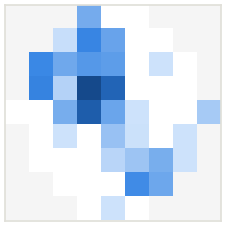
\includegraphics[width=2.0cm]{thumb_out.png}};
  \node[below=2pt of out, text=ink2] {output};
  \draw[-{Stealth[length=6pt]}, line width=1.2pt, cOT] (in) -- node[above=3pt, text=ink] {flow}
    node[below=3pt, text=ink2] {(ODE)} (out);
  \node (jw) [below=1.35cm of out] {
\includegraphics[width=2.0cm]{thumb_jewel.png}};
  \node[below=2pt of jw, text=ink2] {real JEWEL jets};
  \draw[{Stealth[length=5pt]}-{Stealth[length=5pt]}, line width=0.8pt, muted, dashed]
    ([yshift=-14pt]out.south) -- node[right=3pt, text=ink, align=left] {same\\statistics?}
    (jw.north);
  \node[below=1.35cm of in, text=ink2, align=center, text width=2.4cm] {trained on 200k\\PYTHIA + 200k JEWEL
    jets, \textbf{no pairs}};
\end{tikzpicture}
\end{columns}
\end{frame}

% ---------------------------------------------------------------- 3
\begin{frame}{Method and setup}
\begin{columns}[T]
\column{0.5\textwidth}
\textbf{OT flow matching} \refs{1, 2}
\begin{itemize}\setlength\itemsep{0.3em}
\item pair each batch of 256 PYTHIA and 256 JEWEL jets by optimal transport (least change in log energy)
\item learn the velocity along straight lines between pairs (mean-squared-error loss)
\item translate: solve the flow ODE (128 network calls, 6.6 ms per jet)
\item network: the UVCGAN-S generator \refs{3} with a time input, 32M parameters; 2 hours on one A6000
\end{itemize}
\column{0.5\textwidth}
\textbf{Data}: clean jet images, no background
\begin{itemize}\setlength\itemsep{0.3em}
\item PYTHIA 2.6M and JEWEL \refs{4} 870k events; the leading R = 0.4 jet, 53 towers on a 16 $\times$ 16
  grid
\item per sample: 200k training jets, 20k held-out test jets, split by event
\end{itemize}
\vspace{0.4em}
\textbf{References for comparison}
\begin{itemize}\setlength\itemsep{0.3em}
\item the PYTHIA jet, unchanged
\item \keyrj a random JEWEL jet: right distributions, ignores the input
\item a second JEWEL sample: the best possible match
\end{itemize}
\end{columns}
\end{frame}

% ---------------------------------------------------------------- 4
\begin{frame}{Jet $p_T$ spectra}
\begin{center}
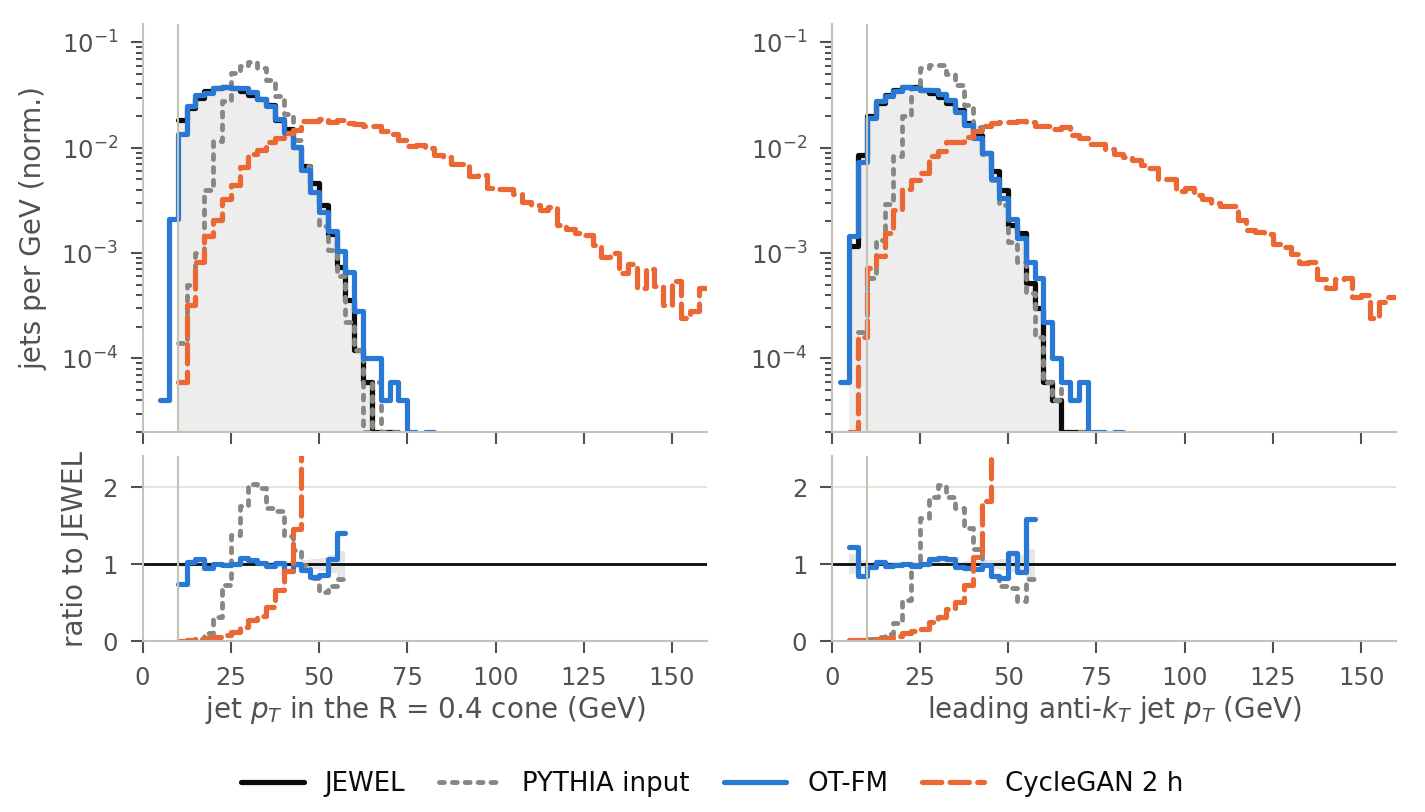
\includegraphics[width=0.7\textwidth]{deck_pt.png}
\end{center}
\vspace{-0.6em}
\begin{itemize}\setlength\itemsep{0.3em}
\item the PYTHIA inputs start near 20 GeV; \ot{} outputs follow the JEWEL spectrum within statistical
  errors from 10 to about 55 GeV, for the cone and for re-found anti-$k_T$ jets
\end{itemize}
\end{frame}

% ---------------------------------------------------------------- 5
\begin{frame}{Jet substructure}
\begin{columns}[c]
\column{0.5\textwidth}
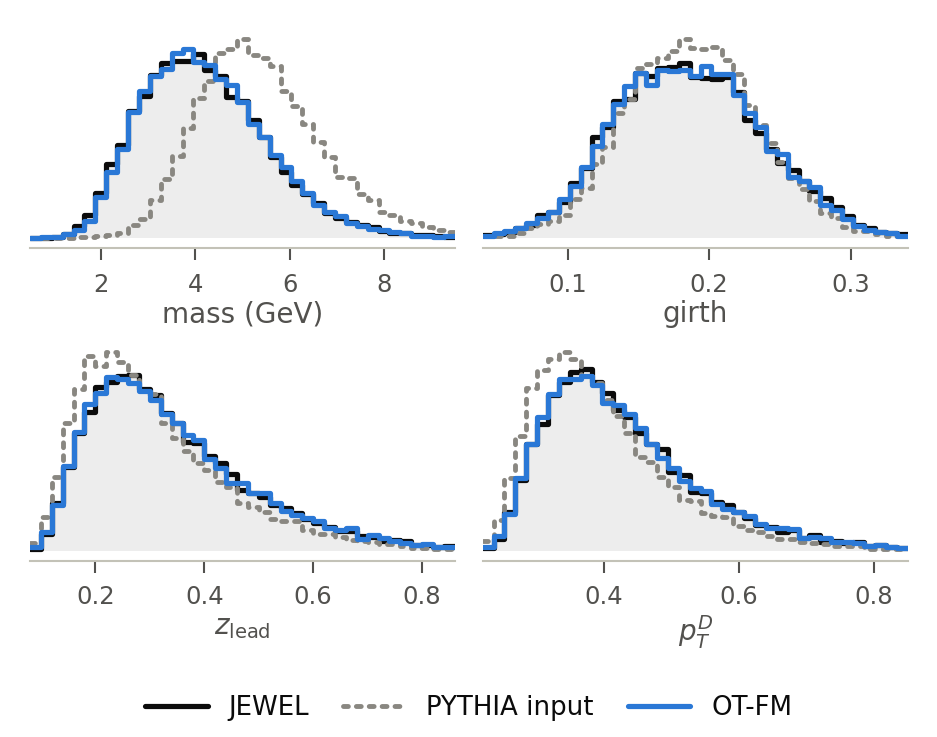
\includegraphics[width=\textwidth]{deck_marginals.png}
\column{0.5\textwidth}
\footnotesize
\scriptsize
\setlength{\tabcolsep}{4pt}
\begin{tabular}{lrrrr}
\toprule
 & JEWEL vs & PYTHIA & \keyrj random & \keyot OT-FM \\
 & JEWEL & input & JEWEL jet &  \\
\midrule
$p_T$ & 0.011 & 0.55 & 0.019 & \textbf{0.025} \\
mass & 0.014 & 0.88 & 0.024 & \textbf{0.021} \\
girth & 0.009 & 0.10 & 0.011 & \textbf{0.012} \\
$z_\mathrm{lead}$ & 0.019 & 0.23 & 0.011 & \textbf{0.008} \\
$p_T^D$ & 0.018 & 0.26 & 0.010 & \textbf{0.010} \\
$z_g$ & 0.012 & 0.034 & 0.005 & \textbf{0.017} \\
$R_g$ & 0.008 & 0.16 & 0.010 & \textbf{0.012} \\
\bottomrule
\end{tabular}

\smallnote{Distance to 20k held-out JEWEL jets (W1 / $\sigma$, lower is better; jets with $p_T \ge$ 10
GeV). Bold: as close as a second JEWEL sample, within 3 standard deviations.}
\vspace{0.6em}
\normalsize
\begin{itemize}\setlength\itemsep{0.3em}
\item \ot{} is as close to JEWEL as a second JEWEL sample in all seven observables
\end{itemize}
\end{columns}
\end{frame}

% ---------------------------------------------------------------- 6
\begin{frame}{Jet shapes at fixed $p_T$}
\begin{center}
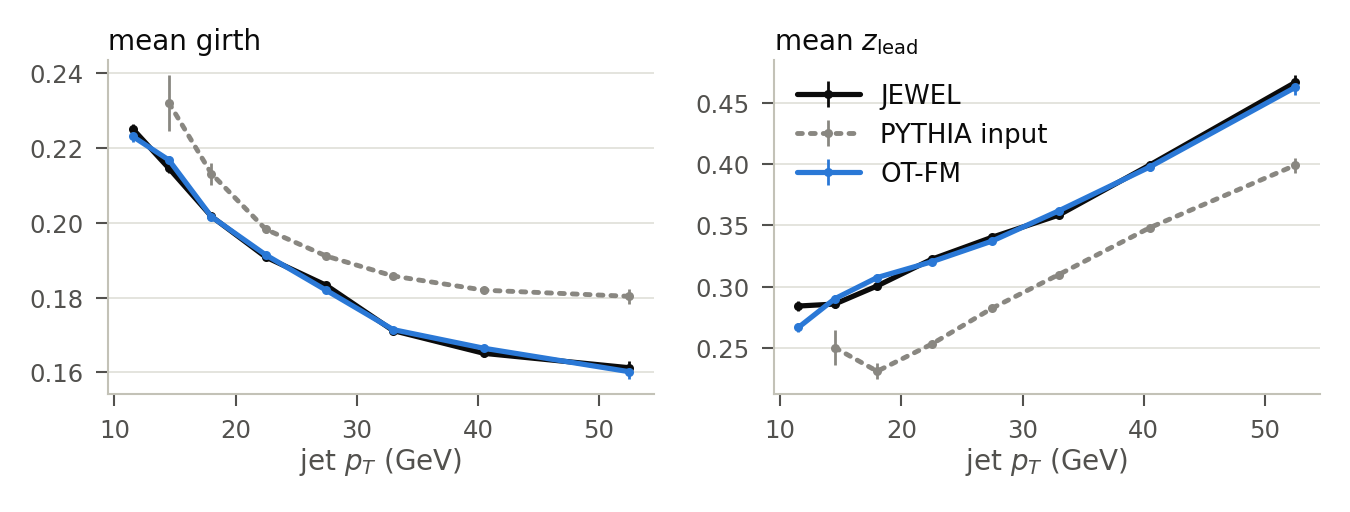
\includegraphics[width=0.8\textwidth]{deck_profiles.png}
\end{center}
\vspace{-0.4em}
\begin{itemize}\setlength\itemsep{0.35em}
\item at the same $p_T$, JEWEL jets are \textbf{narrower} and \textbf{harder} (higher $z_\mathrm{lead}$)
  than PYTHIA jets
\item \ot{} follows both trends in every $p_T$ bin
\end{itemize}
\end{frame}

% ---------------------------------------------------------------- 7
\begin{frame}{How much does each jet change?}
\begin{columns}[c]
\column{0.57\textwidth}
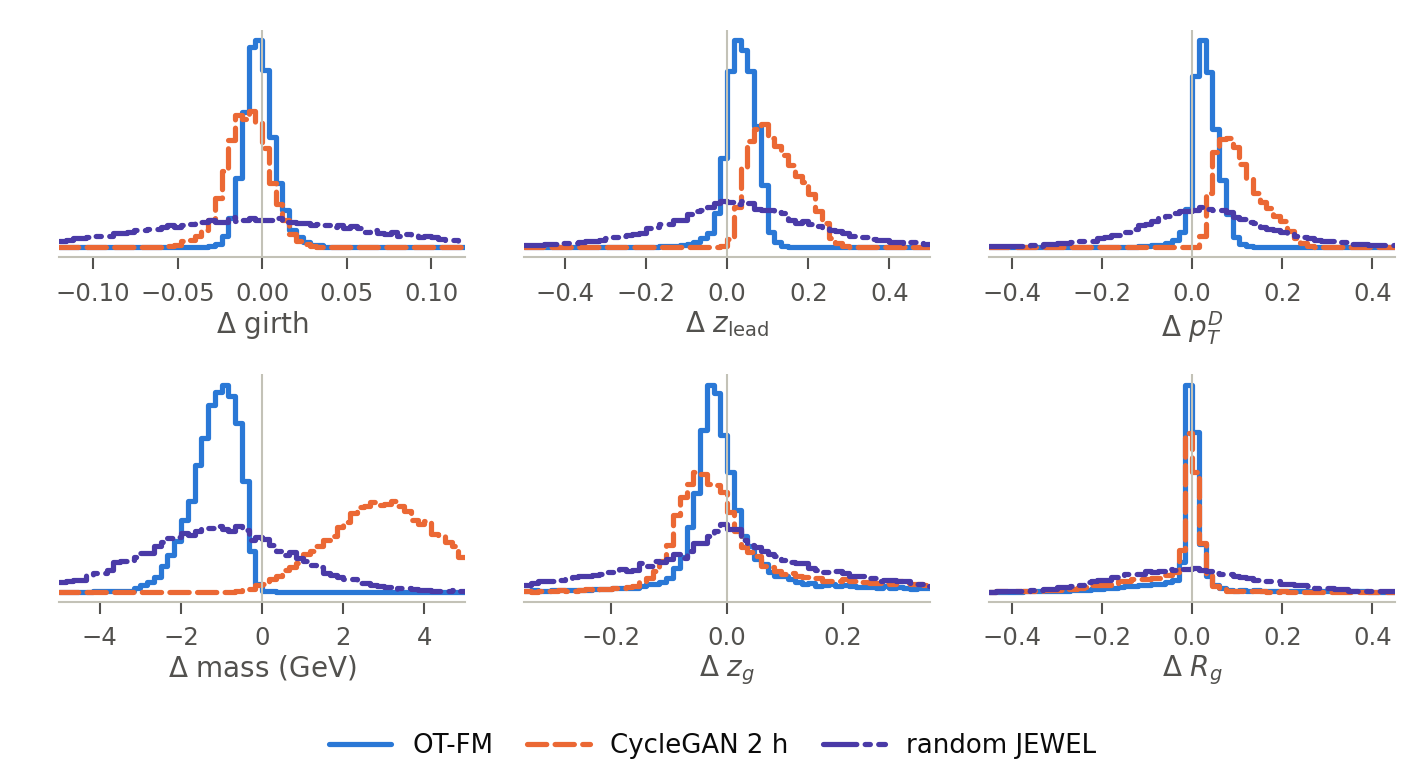
\includegraphics[width=\textwidth]{deck_shape_changes.png}
\column{0.43\textwidth}
\footnotesize
\scriptsize
\setlength{\tabcolsep}{5pt}
\begin{tabular}{lrrr}
\toprule
 & \multicolumn{2}{c}{rms of the change} & \multicolumn{1}{c}{ratio} \\
 & \keyot OT-FM & \keyrj random & random / \\
 &  & JEWEL jet & OT-FM \\
\midrule
girth & 0.009 & 0.069 & 7.4 \\
$z_\mathrm{lead}$ & 0.051 & 0.203 & 4.0 \\
$p_T^D$ & 0.042 & 0.159 & 3.8 \\
mass (GeV) & 1.303 & 2.220 & 1.7 \\
$z_g$ & 0.094 & 0.157 & 1.7 \\
$R_g$ & 0.065 & 0.152 & 2.3 \\
\bottomrule
\end{tabular}

\smallnote{Change = output minus its own input, all 20k test jets.}
\vspace{0.6em}
\normalsize
\begin{itemize}\setlength\itemsep{0.35em}
\item both reach the JEWEL distributions, so their \textbf{average} change is the same (e.g.
  $z_\mathrm{lead}$ +0.03, mass $-1.2$ GeV)
\item \ot{} changes each jet \textbf{1.7-7$\times$ less}: it moves a jet only as far as needed; a random
  JEWEL jet replaces it
\end{itemize}
\end{columns}
\end{frame}

% ---------------------------------------------------------------- 8
\begin{frame}{Output against input, jet by jet}
\begin{columns}[c]
\column{0.56\textwidth}
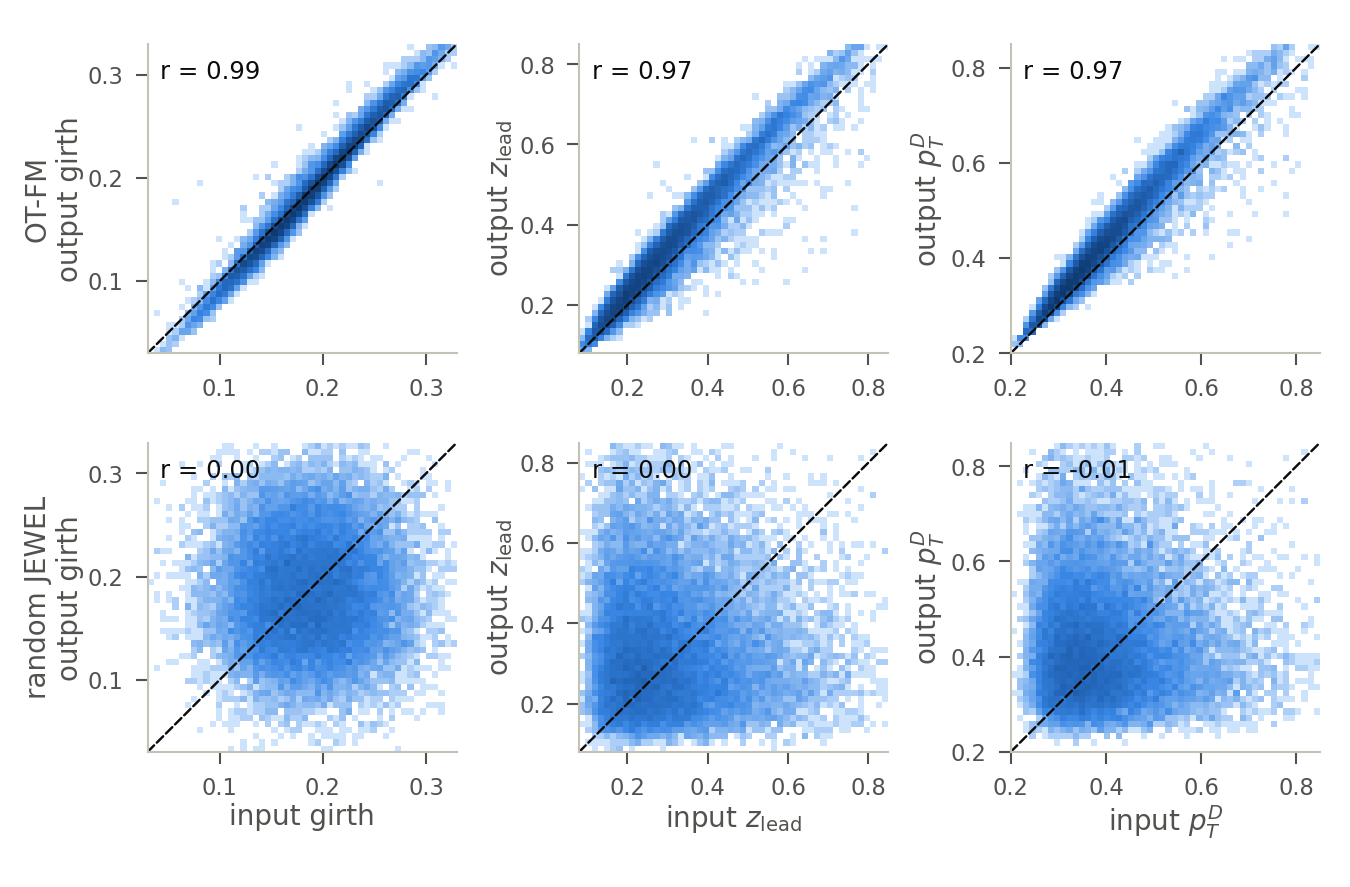
\includegraphics[width=\textwidth]{deck_shape_scatter.png}
\column{0.44\textwidth}
\footnotesize
\scriptsize
\setlength{\tabcolsep}{5pt}
\begin{tabular}{lrr}
\toprule
 & \keyrj random & \keyot OT-FM \\
 & JEWEL jet &  \\
\midrule
$p_T$ & 0.01 & 0.94 \\
girth & 0.00 & 0.99 \\
mass & 0.01 & 0.91 \\
core fraction & 0.00 & 0.99 \\
leading tower & 0.00 & 0.92 \\
\midrule
own input preferred & 50\% & 100\% \\
\bottomrule
\end{tabular}

\smallnote{Input-output correlation, 20k test jets (core: within $\Delta R <$ 0.15). Own input: share of
outputs closer in shape to their own input than to another input jet.}
\vspace{0.5em}
\normalsize
\begin{itemize}\setlength\itemsep{0.3em}
\item \ot{} keeps the ordering of jets and makes each slightly harder ($z_\mathrm{lead}$, $p_T^D$ above
  the diagonal)
\item a random JEWEL jet has no link to its input
\end{itemize}
\end{columns}
\end{frame}

% ---------------------------------------------------------------- 9
\begin{frame}{Examples}
\begin{columns}[c]
\column{0.5\textwidth}
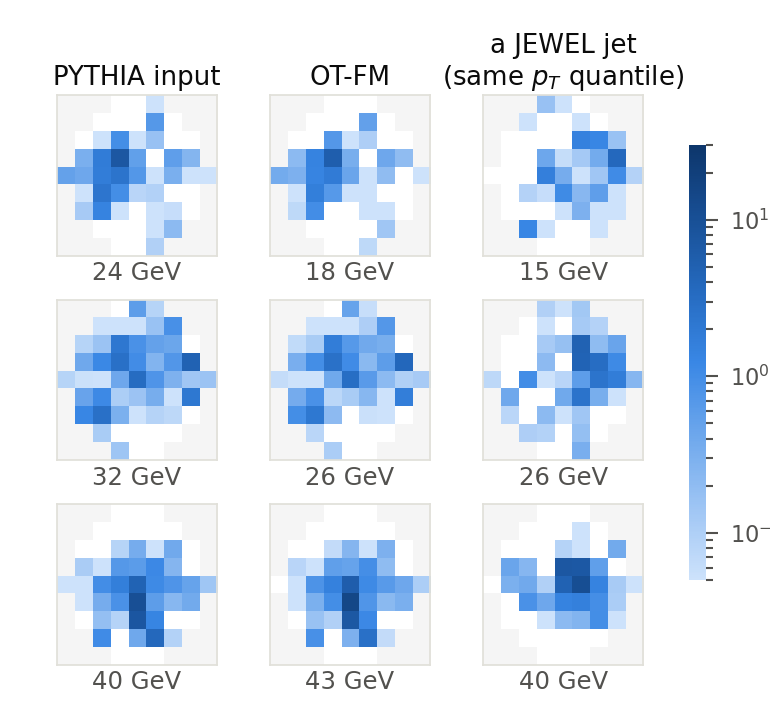
\includegraphics[width=\textwidth]{deck_displays.png}
\column{0.5\textwidth}
\begin{itemize}\setlength\itemsep{0.5em}
\item each output keeps its input's prongs and layout
\item low-$p_T$ jets lose energy; the cores of high-$p_T$ jets get harder
\end{itemize}
\vspace{0.4em}
\smallnote{Fixed held-out inputs at $p_T$ quantiles 0.1, 0.5 and 0.9. The JEWEL jet is a reference at the
same $p_T$ quantile, not a truth.}
\end{columns}
\end{frame}

% ---------------------------------------------------------------- 10
\begin{frame}{Caveat: the $p_T$ change follows the two samples}
\begin{columns}[c]
\column{0.5\textwidth}
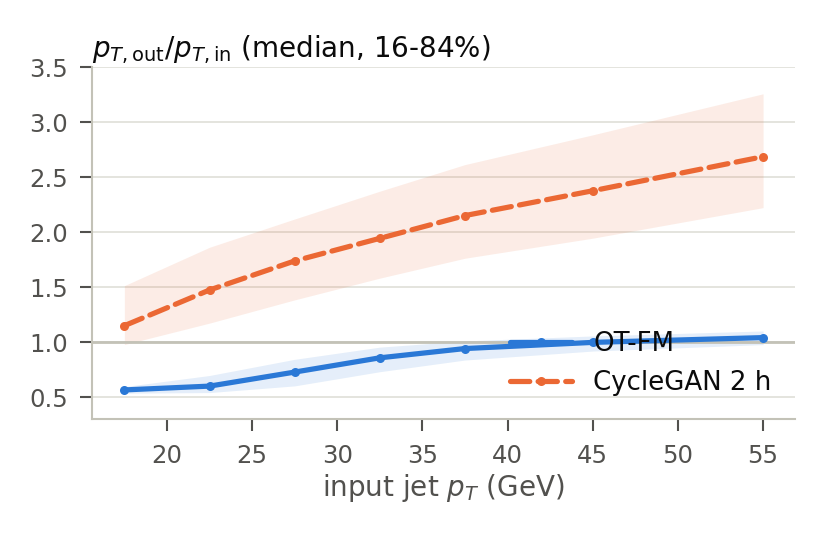
\includegraphics[width=\textwidth]{deck_ptchange.png}
\column{0.5\textwidth}
\begin{itemize}\setlength\itemsep{0.4em}
\item the PYTHIA sample starts near 20 GeV (presumably its generator-level jet requirement); JEWEL
  reaches down to 10 GeV
\item \ot{} lowers 20-25 GeV jets by 40\% and leaves jets above 40 GeV unchanged: a map between two
  differently selected samples, not a quenching mechanism
\end{itemize}
\end{columns}
\end{frame}

% ---------------------------------------------------------------- 11
\begin{frame}{Summary}
\begin{columns}[T]
\column{0.5\textwidth}
\textbf{Shown}
\begin{itemize}\setlength\itemsep{0.4em}
\item trained without pairs in 2 GPU hours, \ot{} produces jets statistically indistinguishable from
  held-out JEWEL: $p_T$, 7 substructure observables, their $p_T$ dependence, re-found jets
\item each output stays tied to its input (correlations 0.91-0.99) and changes 1.7-7$\times$ less than a
  random JEWEL jet would
\end{itemize}
\column{0.5\textwidth}
\textbf{Not shown}
\begin{itemize}\setlength\itemsep{0.4em}
\item a per-jet medium modification: there is no per-jet truth, and optimal transport picks the
  least-change map
\item physics in the $p_T$ shift: it reflects how the samples were selected
\item robustness: one seed
\end{itemize}
\end{columns}
\vspace{1.2em}
\colorbox{wash}{\parbox{0.97\linewidth}{\vspace{0.4em}\hspace{0.3em}\textbf{Next:} train two more seeds.
Does the same PYTHIA jet get the same output, not only the same distributions?\vspace{0.4em}}}

\vspace{0.8em}
\smallnote{Practical: the ODE needs 128 network calls (a 4-step solve lowers the jet $p_T$ too much: mean 22 against 27 GeV); towers that
should be empty get $\sim$0.002 GeV, 0.1\% of the jet energy.}
\end{frame}

% ---------------------------------------------------------------- 12
\begin{frame}{References}
\footnotesize
\begin{enumerate}\setlength\itemsep{0.5em}
\item Y. Lipman, R. T. Q. Chen, H. Ben-Hamu, M. Nickel, M. Le, \emph{Flow Matching for Generative
  Modeling}, ICLR 2023, arXiv:2210.02747
\item A. Tong, K. Fatras, N. Malkin, G. Huguet, Y. Zhang, J. Rector-Brooks, G. Wolf, Y. Bengio,
  \emph{Improving and generalizing flow-based generative models with minibatch optimal transport}
  (OT-CFM), TMLR 2024, arXiv:2302.00482; code: \texttt{github.com/atong01/conditional-flow-matching}
\item \emph{Stratified CycleGAN for unsupervised data decomposition} (UVCGAN-S), arXiv:2510.23717; the
  generator network used here
\item K. C. Zapp, \emph{JEWEL 2.0.0: directions for use}, Eur. Phys. J. C 74 (2014) 2762,
  arXiv:1311.0048
\end{enumerate}
\end{frame}

\end{document}
